\documentclass[11pt]{report}

\usepackage{graphicx}
\usepackage[utf8]{inputenc}


\begin{document}
\title{Virtual Reality}
\author{Maximilian Sieß}
\maketitle

\tableofcontents

%\chapter{Abstract}

\chapter{Introduction}
Virtual Reality is the attempt to use technology, such as head mounted display devices, and computer generated graphics, to allow the user to experience a sense of presence in a virtual environment.  This is used in a wide variety of cases, including but not limited to, entertainment, education, medical therapy, research, and visualization. Virtual Reality, or VR for short, has the potential to fundamentally change the way we experience, and interact with, data and software.

	\section{Definitions}
		\subsection{Virtual Reality}
			Virtual Reality, or VR for short, is the field of computing that aims to create a virtual world, allowing the user to enter, experience and interact with it, via using specific devices to simulate the virtual environment and the feedback it would provide in order to make the experience as real as possible.
			%"Virtual Reality stands for the field of computing which has the objective of creating a virtual world, having one immerse into it and giving one the capability of interacting with this world, while using specific devices to simulate an environment and stimulate one by feedback in order to make the experience as real as possible." 
			\cite{boas13}
			
		\subsection{Immersion}
			Immersion can be differentiated into three different forms. \textit{Engagement}, which has to come from the subject, not the medium. \textit{Engrossment}, which depends on how the software is designed, and is important to affect a subjects emotions, if that should be the intented goal. And lastly \textit{total immersion}, or the sense of presence. Total immersion can be understood as what happens when someone is fully engulfed by a book, movie, or computer game. \cite{Brown:2004:GIG:985921.986048} \\
			It can also, in the case of VR, be taken more literally as the “extent to which a person’s cognitive and perceptual systems are tricked into believing they are somewhere other than their physical location” \cite{Patrick:2000:ULP:332040.332479}

		\subsection{Telepresence}
			To have the experience that one is present at another location than his or her phyiscal one.  This name has been coined by Marvin Minsky in the 1980s. \cite{minsky1980telepresence} While Minsky had in mind that ones actions have consequences at another phsyical location somewhere, Virtual Reality follows the same concept.
			
\chapter{Related Work}
	\section{Head-Mounted Displays}
		Today, the most common form of how Virtual Reality is realized is via head-mounted displays. Goggles with a high density display in it, the same as used in phones. Utilizing special lenses and stereoscopic vision to create a believable view into the virtual environment. \\
		Examples for headsets like these would be the Oculus Rift by Oculus VR and one under the working title Project Morpheus by Sony. Both are very similiar in execution and produce a VR experience of similiar quality. \cite{goradia2014review}
		
		%The concept of Virtual Reality dates back to the 1980s (Citation Needed), and unlike some depiction of it in pop culture at the time, never archived the level of immersion and presence that recent technological advances enable us to. Due to a jump in interest hardware such as the Oculus Rift found funding in recent years. In the case of Oculus, it was via Crowdfunding. But as a result, commercial products from Google, Valve/HTC or Sony have been announced. At the time of writing, none of the mentioned companies have released a commercially available end user product. Oculus Rift has released and sold Developer Kits, which are most frequently used in modern Virtual Reality endeavours.
	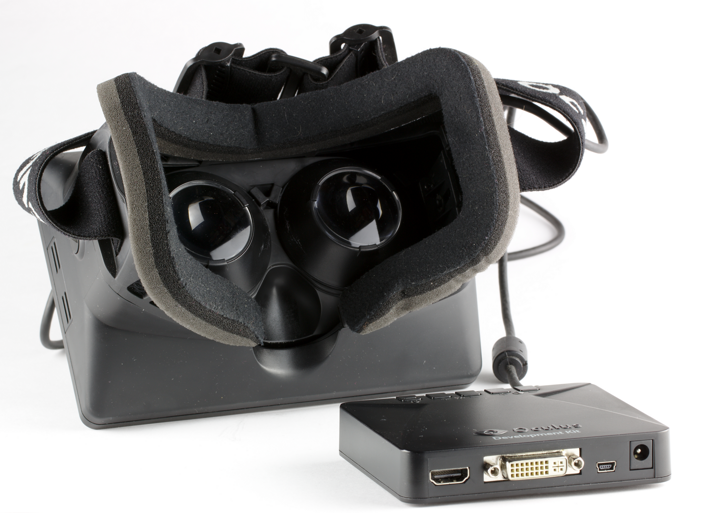
\includegraphics[scale=0.3]{or_small.png}

	\section{Software}
		Programming software for virtual reality does not differ much from regular computer graphics programming. Most commercial vendors offer their own API that helps translating a virtual camera to a two camera 3D setup. It was found however, that how the camera is used is imperitive to not give the user of the virtual reality headsead motion sickness. For example, moving the camera without the user moving their head was resulted in severly negative feedback from the test subjects.
		
		The Oculus Rift Best Practices Manual states that "Acceleration creates a mismatch among your visual, vestibular, and proprioceptive senses; minimize the duration and frequency of such conflicts. Make accelerations as short (preferably instantaneous) and infrequent as you can." \cite{yao2014oculus}
	
	\section{Input Devices}
	With headmounted displays, vision, the groundwork for a feeling of presence in virtual reality, is laid out. Headsets or surround sound systems have been shown to suffice for the audio representation of the virtual environment.\\
	Moving around naturally has proven difficult, however. While video game demos often use a gamepad, it is less than ideal for upholding a sense of presence. Products, such as the XYZ try to enable free movement in virtual reality.



	%\section{Entertainment}
	%Oculus rift, Valve, Project Morpheus - VIDJA GAMES!
	
	%\section{Education}
	%Look at papers you downloaded
	
	%\section{Therapy}
	%Look at papers or download more!
	
	%\section{Research}
	%Papers!
	
	%\section{Visualization}
	%You know, like for surgery, architecture and stuffs.


\chapter{Discussion}
%How helpful is it now? Will it be real reality soon? how soon? absolute presence is not possible with just a headmount set, so wtf Valve, where is my absolute-immersion-set that lets me LittlePip and shoot down some raiders, eh?


%\chapter{Conclusion}

%\chapter{References}

%\chapter{Appendix}

\bibliographystyle{plain}
\bibliography{vr_bib}

\chapter{notes}
Overview of VR - Definition of Virtual Reality, Immersion, Perception and Telepresence. 
"Virtual Reality development were manly found in the military and academic research until technologies became more cost-effective."
Oh yeah, also input devices are a big factor, shit. Gloves, wands (like the Wii or PS Move) and computer vision.
Also, military wants VR too, woops.
	
Best Practices - VR is hard and every single minor detail is super fucking important so listen to us, fuckers!
"Acceleration creates a mismatch among your visual, vestibular, and proprioceptive senses;
minimize the duration and frequency of such conflicts. Make accelerations as short (preferably
instantaneous) and infrequent as you can."

arm therapy - Use VR to distract patience from pain while their burn wounds are treated. Seems to work!

unwanted sideeffects - cybersickness or simulator sickness

supply chain eduction - use a VR game to teach

serious games for ancient manuscripts - making vr games about really old books ? Allowing people to experience... reading a really old book.

\end{document}
